\documentclass[a4paper, 12pt]{article}
\usepackage{geometry}
\geometry{a4paper,
total={170mm,257mm},left=2cm,right=2cm,
top=2cm,bottom=2cm}

\usepackage{mathtext}
\usepackage{amsmath}
\usepackage[utf8]{inputenc}
\usepackage[english,russian]{babel}
\usepackage{graphicx, float}
\usepackage{tabularx, colortbl}
\usepackage{caption}
\usepackage{wrapfig}

\captionsetup{labelsep=period}

\newcommand{\parag}[1]{\paragraph*{#1:}}
\DeclareSymbolFont{T2Aletters}{T2A}{cmr}{m}{it}
\newcounter{Points}
\setcounter{Points}{1}
\newcommand{\point}{\arabic{Points}. \addtocounter{Points}{1}}
\newcolumntype{C}{>{\centering\arraybackslash}X}

\author{Калинин Даниил, Б01-110}
\date{\today}
\title{Лабораторная работа 1.3.1\\Определение модуля Юнга на основе исследования деформаций растяжения и изгиба}

\begin{document}
\maketitle

\parag {Цель работы}
экспериментально получить зависимость между напряжением и деформацией (закон Гука) для двух простейших напряженных состояний упругих тел: одноосного растяжения и чистого изгиба; по результатам измерений вычислить модуль Юнга.

\parag {В работе используются}
В работе используются: в первой части — прибор Лермантова,проволока из исследуемого материала, зрительная труба со шкалой, набор грузов, микрометр, рулетка; во второй части — стойка для изгибания балки, индикатор для измерения величины прогиба, набор исследуемых стержней, грузы, линейка, штангенциркуль

\parag {Теоритическая справка} ~\\

\begin{wrapfigure}{l}{7cm}
    \centering
    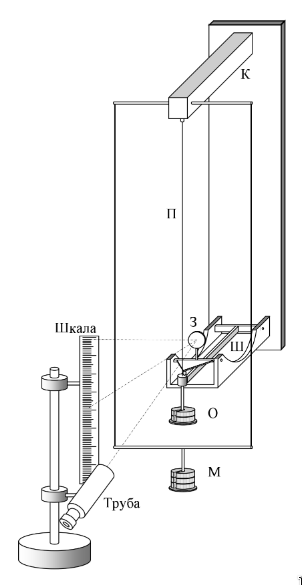
\includegraphics[width=\linewidth]{lermantov.png}
	\caption{Прибор Лермантова}
    \label{pic:lermantov}
\end{wrapfigure}

Для определения модуля Юнга используется прибор Лермантова, схема которого изображена на рис. 1. Верхний конец проволоки П, изготовленной из исследуемого материала, прикреплен к консоли К, а нижний — к цилиндру, которым окаичиваотся шарнирный кронштейн Ш. На этот же цилиндр опирается рычаг r, связанный с зеркальцем 3. Таким образом, удлинение проволоки можжио измерить по углу поворота зеркальца.
Натяжение проволоки можно менять, перекладывая грузы с площадки М на площадку О и наоборот. Такая систома позволяет исключить влияние деформации кронштейна К на точность измерений, так как нагрузка ма нем вос время остается постоянной.
При проведении эксперимента следует иметь в виду, что проволока. При отсутствии нагрузки всегда несколько изогиута, что не может не сказаться па результатах, особенно при небольших нагрузках. Проволока вначале не столько растягивается, сколько распрямляется. \clearpage

\begin{figure}{l}
    \centering
    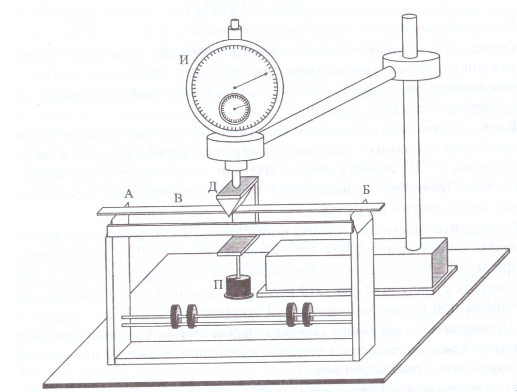
\includegraphics[width=\linewidth]{setup2.png}
	\caption{Установка для измерения модуля Юнга}
    \label{pic:setup2}
\end{figure}

Экспериментальная установка состоит из прочной стойки с опорными призами А и В (рис. 2). На ребра призм опирается исследуемый стержепь (балка) В. В середине стержня на призме Д подвешена площадка И с грузами. Измерять стрелу прогиба можно с помощью индикатора И, укрепляемого на отдельной штанге. Полный оборот большой стрелки индикатора соответствует 1 мм и одному делению малого циферблада.


\parag {Обработка результатов эксперимента}~\\

\point \textbf{Определение модуля Юнга по измерениям растяжения проволоки.}

\point Запишем погрешности измерительных приборов в таблицу \ref{tabl:inaccs}.

\begin{table}[H]
    \centering
    \begin{tabular}{|l|l|l|}
    \hline
           & Прибор         & Погрешность         \\ \hline
    1      & Линейка        & $\sigma = 0.5$ мм.  \\ \hline
    2      & Штангенциркуль & $\sigma = 0.05$ мм. \\ \hline
    \end{tabular}
	\caption{Погрешности}
    \label{tabl:inaccs}
\end{table}

\point Измерим параметры установки, результаты занесем в таблицу \ref{tabl:lermantov_data}

\begin{table}
    \centering
    \begin{tabular}{|l|l|}
    \hline
           $\bar{d}$ проволоки   & $0.73  \pm 0.05$ мм.          \\ \hline
           $l$ проволоки         & $176.4 \pm 0.05$ cм.          \\ \hline
           $h$ проволоки         & $137.1 \pm 0.05$ cм.          \\ \hline
           $r$ рычага            & $13    \pm 0.05$ cм.          \\ \hline
    \end{tabular}
    
	\caption{Параметры установки}
    \label{tabl:lermantov_data}
\end{table}

\point Определим максимальную рабочую нагрузку:
\[
    F_{max} = 900 \cdot 0.30 \frac{\pi d^2}{4} = 44.8 Н.
\]

Таким образом, проволоку нельзя нагружать больше, чем на 4.5 кг.

\point Направляем зрительную трубу на зеркальце так, чтобы мы четко видели шкалу, тогда свет от шкалы будет падать примерно перпендикулярно шкале на зеркало, поэтому
\[
    \Delta l =\dfrac{nr}{2h}
\]
\[
    \sigma_{\Delta l} = \Delta l\sqrt{\left( \dfrac{\sigma_{n}}{n}\right)^2 + \left(\dfrac{\sigma_d}{d}\right)^2+\left(\dfrac{\sigma_h}{h}\right)^2} 
\]

Проведем три эксперимента по определению растяжения проволоки, вначале постепенно добавляя, а затем постепенно убирая грузы с площадки. Результаты занесем в таблицу \ref{tabl:data1}

\begin{table}
    \centering
    \begin{tabular}{| p{5em} | p{5em} | p{5em} | p{5em} | p{5em}| p{5em} | p{5em} |}
        \hline
        \multicolumn{2}{|c|}{Эксперимент № 1} & \multicolumn{2}{|c|}{Эксперимент № 2} & \multicolumn{2}{|c|}{Эксперимент № 3} \\ \hline 
        Деление на линейке & Суммарная масса грузов, гр. & Деление на линейке & Суммарная масса грузов, гр. & Деление на линейке & Суммарная масса грузов, гр. \\ \hline
        6.5  & 245.8  & 6.4  & 245.8  & 6    & 245.8  \\ \hline
        8    & 491.9  & 7.5  & 491.9  & 8.1  & 491.9  \\ \hline
        9    & 737.4  & 8.7  & 737.4  & 9    & 737.4  \\ \hline
        10.1 & 983.5  & 9.9  & 983.5  & 10.3 & 983.5  \\ \hline
        11.2 & 1229.2 & 11   & 1229.2 & 11.4 & 1229.2 \\ \hline
        12.3 & 1474.9 & 12.3 & 1474.9 & 12.  & 1474.9 \\ \hline
        13.6 & 1720.4 & 13.1 & 1720.4 & 13.5 & 1720.4 \\ \hline
        15   & 1965.8 & 14.3 & 1965.8 & 14.3 & 1965.8 \\ \hline
        16   & 2211.4 & 15.4 & 2211.4 & 15.9 & 2211.4 \\ \hline
        17.1 & 2457   & 16.6 & 2457   & 16.5 & 2457   \\ \hline
        17.1 & 2457   & 16.6 & 2457   & 16.5 & 2457   \\ \hline
        15.8 & 2211.4 & 15.3 & 2211.4 & 14.7 & 2211.4 \\ \hline
        14.4 & 1965.8 & 14.4 & 1965.8 & 13.6 & 1965.8 \\ \hline
        13.2 & 1720.4 & 13   & 1720.4 & 12.4 & 1720.4 \\ \hline
        12.3 & 1474.9 & 11.8 & 1474.9 & 11.3 & 1474.9 \\ \hline
        11.2 & 1229.2 & 10.7 & 1229.2 & 10.2 & 1229.2 \\ \hline
        10.1 & 983.5  & 9.7  & 983.5  & 9    & 983.5  \\ \hline
        8.7  & 737.4  & 8.5  & 737.4  & 7.9  & 737.4  \\ \hline
        7.5  & 491.9  & 7.2  & 491.9  & 6.6  & 491.9  \\ \hline
        6.4  & 245.8  & 5.9  & 245.8  & 5.4  & 245.8  \\ \hline
    \end{tabular}
    \caption{Результаты экспериментов с первой установкой}
    \label{tabl:data1}
\end{table}

По полученным данным вычислим удлинение проволоки и погрешность ее вычисления. Результаты обработки первого эксперимента приведены в таблице \ref{tabl:data2}

\begin{table}
    \centering
    \begin{tabular}{|p{4em}|p{6em}||p{4em}|p{6em}||p{4em}|p{6em}|p{4em}|}
        \hline
        $\Delta l$ в первом эксперименте, см & Погрешность $\sigma_{\Delta l_1}$, см & $\Delta l$ во втором эксперименте, см  & Погрешность $\sigma_{\Delta l_2}$, см & $\Delta l$ в третьем эксперименте, см & Погрешность $\sigma_{\Delta l_3}$, см & масса грузов г. \\ \hline
        0.31 & 0.07 & 0.30 & 0.07  & 0.28 & 0.06  & 245.800 	 \\ \hline
        0.38 & 0.07 & 0.36 & 0.07  & 0.38 & 0.07  & 491.900 	 \\ \hline
        0.43 & 0.08 & 0.41 & 0.08  & 0.43 & 0.08  & 737.400 	 \\ \hline
        0.48 & 0.08 & 0.47 & 0.08  & 0.49 & 0.08  & 983.500 	 \\ \hline
        0.53 & 0.09 & 0.52 & 0.09  & 0.54 & 0.09  & 1229.200 	 \\ \hline
        0.58 & 0.09 & 0.58 & 0.09  & 0.57 & 0.09  & 1474.900 	 \\ \hline
        0.64 & 0.10 & 0.62 & 0.10  & 0.64 & 0.10  & 1720.400 	 \\ \hline
        0.71 & 0.11 & 0.68 & 0.11  & 0.68 & 0.11  & 1965.800 	 \\ \hline
        0.76 & 0.12 & 0.73 & 0.11  & 0.75 & 0.11  & 2211.400 	 \\ \hline
        0.81 & 0.12 & 0.79 & 0.12  & 0.78 & 0.12  & 2457.000 	 \\ \hline
        0.81 & 0.12 & 0.79 & 0.12  & 0.78 & 0.12  & 2457.000 	 \\ \hline
        0.75 & 0.11 & 0.73 & 0.11  & 0.70 & 0.11  & 2211.400 	 \\ \hline
        0.68 & 0.11 & 0.68 & 0.11  & 0.64 & 0.10  & 1965.800 	 \\ \hline
        0.63 & 0.10 & 0.62 & 0.10  & 0.59 & 0.09  & 1720.400 	 \\ \hline
        0.58 & 0.09 & 0.56 & 0.09  & 0.54 & 0.09  & 1474.900 	 \\ \hline
        0.53 & 0.09 & 0.51 & 0.09  & 0.48 & 0.08  & 1229.200 	 \\ \hline
        0.48 & 0.08 & 0.46 & 0.08  & 0.43 & 0.08  & 983.500 	 \\ \hline
        0.41 & 0.08 & 0.40 & 0.07  & 0.37 & 0.07  & 737.400 	 \\ \hline
        0.36 & 0.07 & 0.34 & 0.07  & 0.31 & 0.07  & 491.900 	 \\ \hline
        0.30 & 0.07 & 0.28 & 0.06  & 0.26 & 0.06  & 245.800 	 \\ \hline
    \end{tabular}
    \caption{Результаты обработки экспериментов}
    \label{tabl:data2}
\end{table}

\point Построим графики зависимости удлинения проволоки от нагрузки для каждого из трех экспериментов, результаты приведем в графиках \ref{pic:graph1}, \ref{pic:graph2}, \ref{pic:graph3}

В недеформированном состоянии проволока, как правило, изогнута, и при малых нагрузках её "удлинение" определяется не растяжением, а выпрямлением. Найдем уравнение получившийся прямой по МНК. По наклону прямой определим жесткость проволоки, а по ней - модуль Юнга. Начальный участок графика при обработке следует исключить.

\begin{figure}[!h]
    \centering
    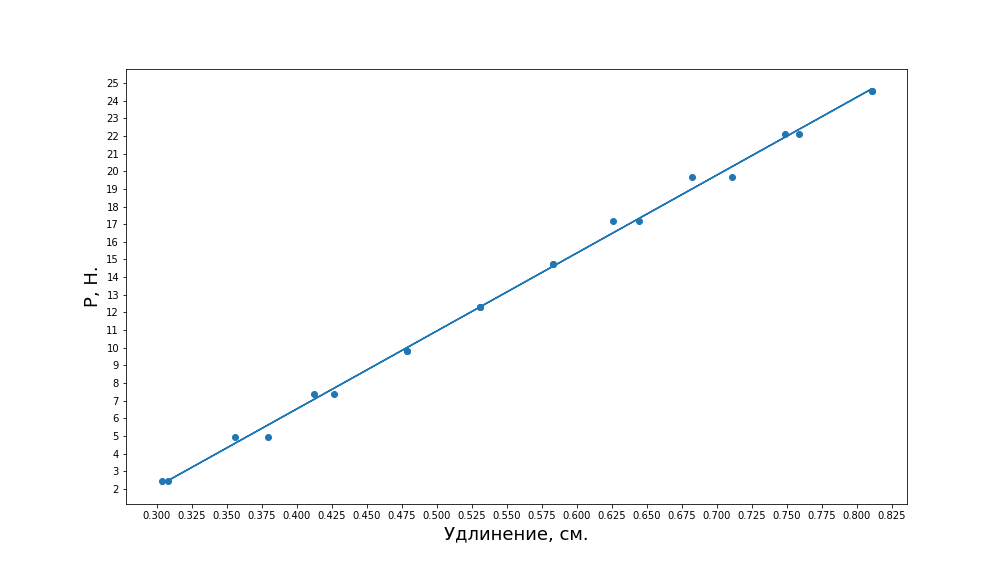
\includegraphics[width=\linewidth]{ex1.png}
    \caption{Первый эксперимент}
    \label{pic:graph1}
\end{figure}

\begin{figure}[!h]
    \centering
    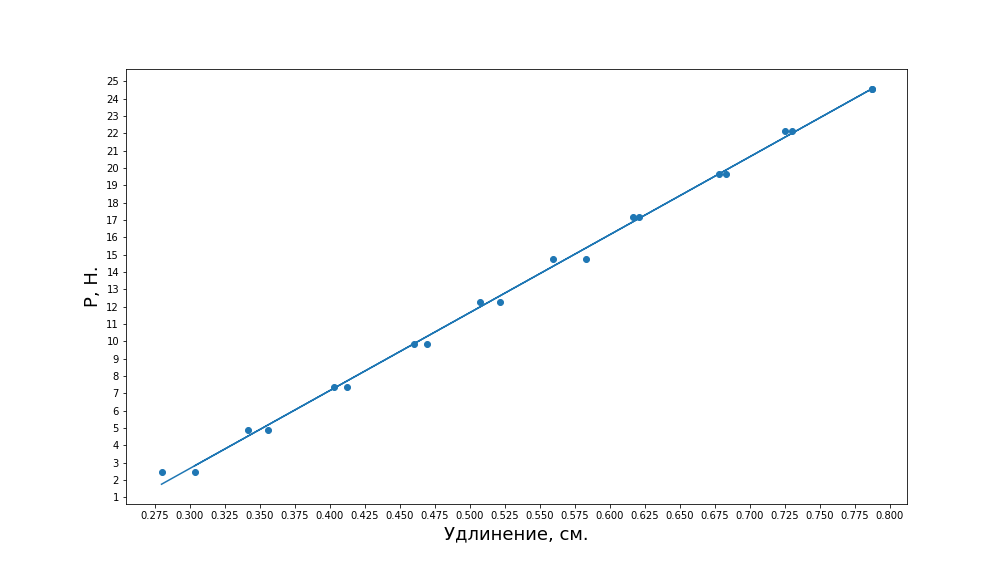
\includegraphics[width=\linewidth]{ex2.png}
    \caption{Второй эксперимент}
    \label{pic:graph2}
\end{figure}

\begin{figure}[!h]
    \centering
    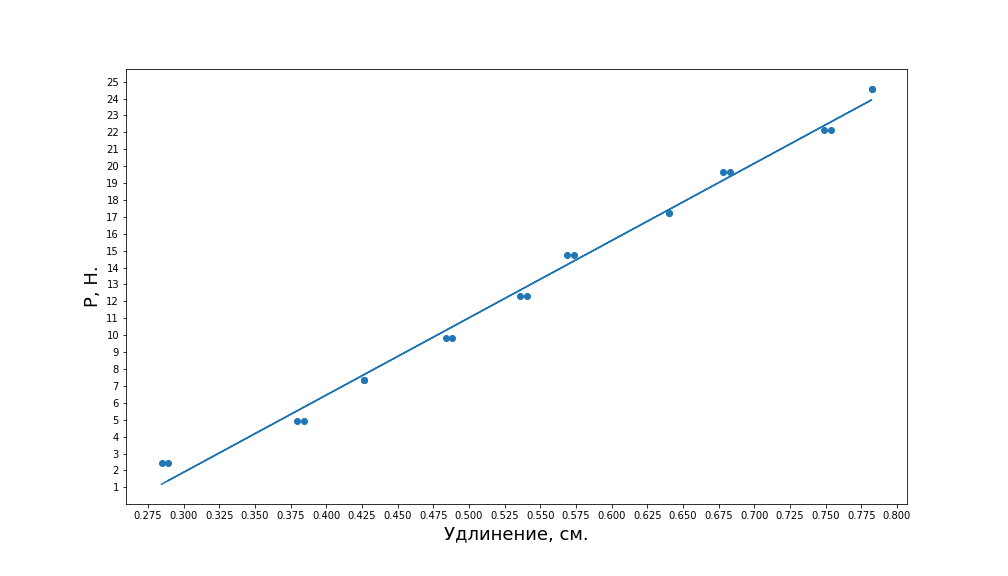
\includegraphics[width=\linewidth]{ex3.png}
    \caption{Третий эксперимент}
    \label{pic:graph3}
\end{figure}


По найденной графически жёсткости проволоки найдем модуль Юнга по формуле
\[E = \dfrac{k \cdot  l_0}{S}\]
\[\sigma_E = \sqrt{\left( \dfrac{\sigma_{k}}{k} \right)^2 + \left( \dfrac{\sigma_{S}}{S} \right)^2 + \left( \dfrac{\sigma_{l_0}}{l_0} \right)^2 }\]

Результаты занесем в таблицу \ref{tabl:res1}

\begin{table}[H]
    \centering
    \begin{tabular}{|c|c|c|c|}
        \hline
         & Значение&$\sigma$&$\varepsilon$\\
        \hline
        $\bar{k}$ & $4.423 \cdot  10^3$ $H/см$ & $0,043 \cdot  10^3$ $Н/м$ & 0,009 \\
        \hline
        $\bar{E}$ & $1.86  \cdot   10^{9}$ $Н/см^2$ & $ 0.5 \cdot  10^{8}$ $Н/см^2$ & 0,05 \\
        \hline
    \end{tabular}
    \caption{Значения k и E}
    \label{tabl:res1}
\end{table}

~\\
\point \textbf{Определение модуля Юнга по измерениям изгиба бруска.}

\point Измерим параметры бруска:
$\bar{l} = 50 \pm 0.05 см$
$\bar{a} = 2 \pm 0.05 см$
$\bar{b} = 1 \pm 0.05 см$

\point Кладем деревянную балку так, чтобы Д было в центре и фиксируем зависимость $y_{max}$ от $P$. Затем переворачиваем балку на 180 градусов, проводим тот же эксперимент. Резльутат заносим в таблицу \ref{tabl:wood1}

\begin{table}
    \centering
    \begin{tabular}{|l | l|}
        \hline 
        $y_{max}$, мм & Суммарная масса грузов, г. \\ \hline 
        0.76 & 504.5  \\ \hline
        1.56 & 1006   \\ \hline
        2.30 & 1509   \\ \hline
        3.4  & 1991.5 \\ \hline
        3.74 & 2455.1 \\ \hline
        4.43 & 2951.3 \\ \hline
        4.43 & 2951.3 \\ \hline
        3.81 & 2455.1 \\ \hline
        3.5  & 1991.5 \\ \hline
        2.4  & 1509   \\ \hline
        1.62 & 1006   \\ \hline
        0.84 & 504.5  \\ \hline

        \multicolumn{2}{|c|}{Перевернутый брусок} \\ \hline

        0.79 & 504.5  \\ \hline
        1.58 & 1006   \\ \hline
        2.36 & 1509   \\ \hline
        3.13 & 1991.5 \\ \hline
        3.86 & 2455.1 \\ \hline
        4.64 & 2951.3 \\ \hline
        4.64 & 2951.3 \\ \hline
        3.92 & 2455.1 \\ \hline
        3.22 & 1991.5 \\ \hline
        2.49 & 1509   \\ \hline
        1.70 & 1006   \\ \hline
        0.94 & 504.5  \\ \hline
    \end{tabular}
    \caption{Деревянный брусок}
    \label{tabl:wood1}
\end{table}

\point Сместим деревянную балку на 3 мм. влево, проведем тот же эксперимент. Результат занесем в таблицу \ref{tabl:wood2}

% 3й, смещаем влево на три миллиметра
\begin{table}[!h]
    \centering
    \begin{tabular}{|l | l|}
        \hline 
        $y_{max}$, мм & Суммарная масса грузов, г. \\ \hline 
        0.8  & 504.5  \\ \hline
        1.29 & 1006   \\ \hline
        2.83 & 1509   \\ \hline
        3.57 & 1991.5 \\ \hline
        3.77 & 2455.1 \\ \hline
        4.49 & 2951.3 \\ \hline
        4.59 & 2951.3 \\ \hline
        3.87 & 2455.1 \\ \hline
        3.17 & 1991.5 \\ \hline
        2.43 & 1509   \\ \hline
        1.69 & 1006   \\ \hline
        0.90 & 504.5  \\ \hline
    \end{tabular}
    \caption{Деревянный брусок, смещенный влево}
    \label{tabl:wood2}
\end{table}

\point Возьмем брусок из латуни, проделаем с ним тот же эксперимент. Затем перевернем его на 180 градусов и повторим то же самое. Результаты измерений занесем в таблицу \ref{tabl:iron}.

\begin{table}[!h]
    \centering
    \begin{tabular}{|l | l|}
        \hline 
        $y_{max}$, мм & Суммарная масса грузов, г. \\ \hline 
        1.26 & 504.5  \\ \hline
        2.5  & 1006   \\ \hline
        3.70 & 1509   \\ \hline
        4.95 & 1991.5 \\ \hline
        6.8  & 2455.1 \\ \hline
        7.33 & 2951.3 \\ \hline
        7.33 & 2951.3 \\ \hline
        6.8  & 2455.1 \\ \hline
        4.93 & 1991.5 \\ \hline
        3.73 & 1509   \\ \hline
        2.49 & 1006   \\ \hline
        1.26 & 504.5  \\ \hline

        \multicolumn{2}{|c|}{Перевернутый брусок} \\ \hline
        
        1.27 & 504.5  \\ \hline
        2.5  & 1006   \\ \hline
        3.74 & 1509   \\ \hline
        4.94 & 1991.5 \\ \hline
        6.08 & 2455.1 \\ \hline
        7.30 & 2951.3 \\ \hline
        7.30 & 2951.3 \\ \hline
        6.08 & 2455.1 \\ \hline
        4.94 & 1991.5 \\ \hline
        3.75 & 1509   \\ \hline
        2.51 & 1006   \\ \hline
        1.30 & 504.5  \\ \hline
    \end{tabular}
    \caption{Металлический брусок}
    \label{tabl:iron}
\end{table}

\point По полученным данным построим графики зависимости $y_{max}$ от $P$: \ref{pic:wood}, \ref{pic:wood_moved}, \ref{pic:metal}

\begin{figure}[!h]
    \centering
    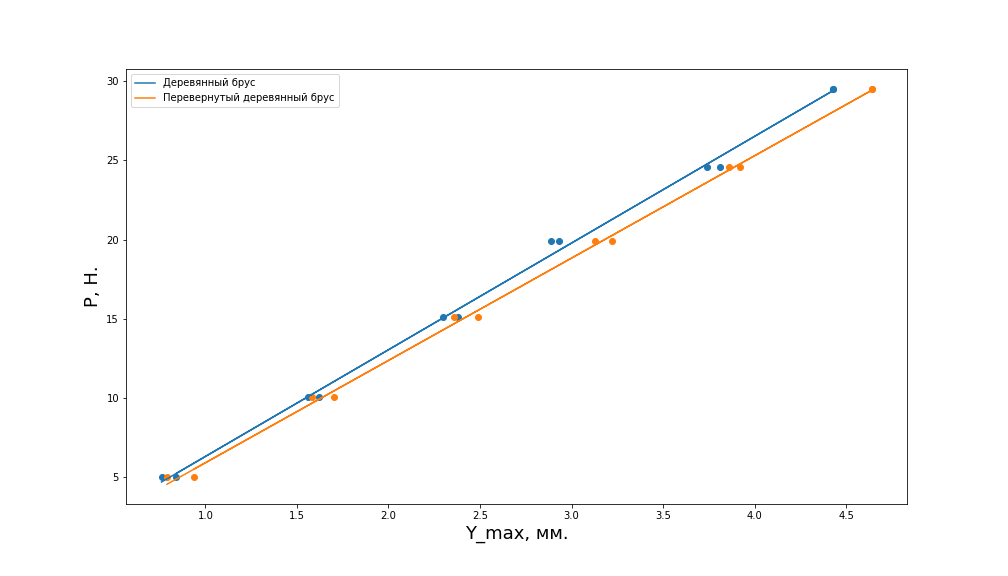
\includegraphics[width=\linewidth]{wood.png}
    \caption{Деревянный брус}
    \label{pic:wood}
\end{figure}

\begin{figure}[!h]
    \centering
    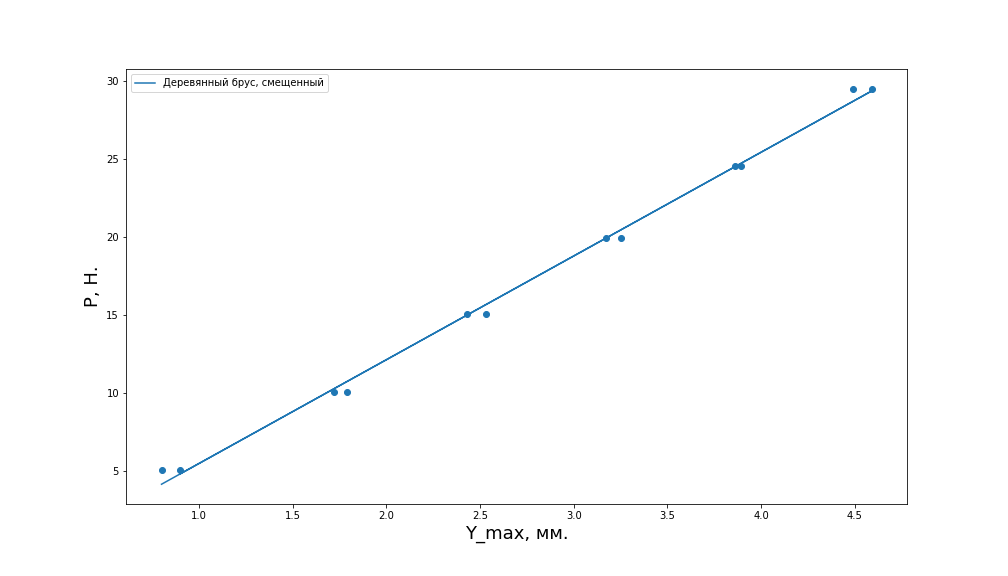
\includegraphics[width=\linewidth]{wood_moved.png}
    \caption{Смещенный деревянный брус }
    \label{pic:wood_moved}
\end{figure}

\begin{figure}[!h]
    \centering
    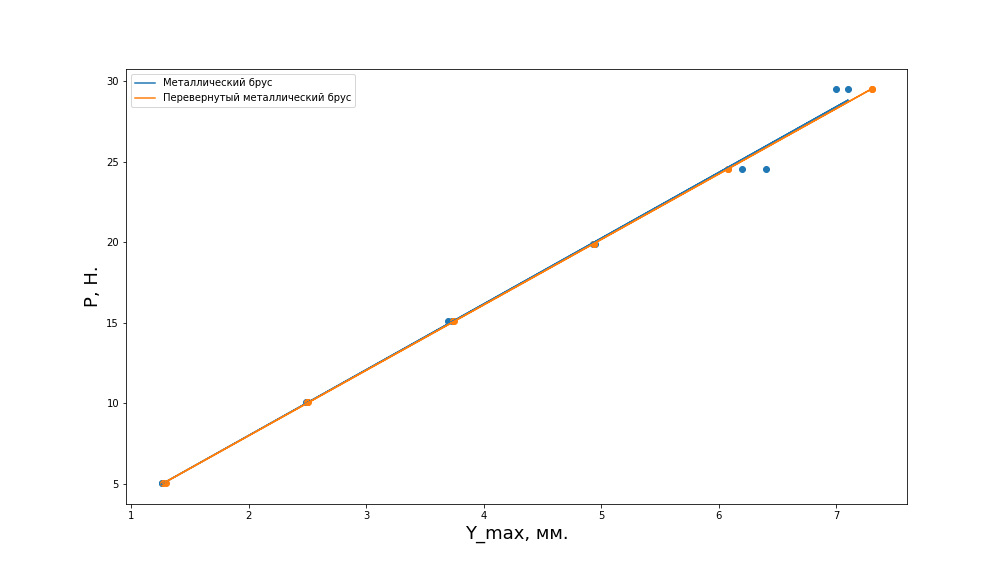
\includegraphics[width=\linewidth]{metal.png}
    \caption{Латунный брус}
    \label{pic:metal}
\end{figure}

Из графиков найдем коэффициенты наклона прямых, расчитаем модуль Юнга брусков по формуле:
\[
    E = \dfrac{Pl^3}{4ab^3y_{max}}
\]
\[
    \sigma_E = \sqrt{3 \left( \dfrac{\sigma_{l}}{l} \right)^2 + \left( \dfrac{\sigma_{P/y_{max}}}{P/y_{max}} \right)^2 + \left( \dfrac{\sigma_{a}}{a} \right)^2 + 3 \left( \dfrac{\sigma_{b}}{b} \right)^2}
\]

Резльутаты занесем в таблицу \ref{tabl:res2}


\begin{table}[H]
    \centering
    \begin{tabular}{|c|c|c|c|}
        \hline
         & Значение&$\sigma$&$\varepsilon$\\
        \hline
        \multicolumn{4}{|c|}{Деревянный брус} \\
        \hline
        $\bar{k}$ & $6.61$ $H/мм$ & $0.745$ $Н/мм$ & $0.11$ \\
        \hline       
        $\bar{E}$ & $1.034 \cdot 10^5$ $Н/мм^2$ & $ 0.03 \cdot 10^5$ $Н/мм^2$ & $0.03$ \\\hline

        \multicolumn{4}{|c|}{Металлический брус} \\
        \hline
        $\bar{k}$ & $4.07$ $H/мм$ & $0.392$ $Н/мм$ & $0.09$ \\
        \hline       
        $\bar{E}$ & $9.47 \cdot 10^{5}$ $Н/мм^2$ & $ 0.02 \cdot  10^{5}$ $Н/см^2$ & 0,022 \\ \hline
    \end{tabular}
    \caption{Значения k и E}
    \label{tabl:res2}
\end{table}


\parag {Заключение} ~\\
В ходе работы мы измерили модуль Юнга проволови и двух брусков. Построили графики зависимости растяжения от силы воздействия. Кроме того, мы посчитали погрешности расчитанных величин, их значения получились приемлемыми. Главное, что в ходе работы мы получили удовольствие и узнали что-то новое.
\end{document}
